\chapter{DISCUSSION}
\label{chap-five}

	\section{Classifiers}
		Classification accuracies for both intra-subject and inter-subject classification tests are generally high for Neural Networks and SVMs compared to Mahalanobis Distance. To understand the reason for differing performances of algorithms, we conducted the Henze-Zirkler's Multivariate Normality Test \cite{HZ} \cite{HZart}. The Henze-Zirkler test is based on a non-negative functional distance that measures the distance between two distribution functions. If the data is multivariate normal, the test statistic HZ is approximately lognormally distributed. We calculate the mean, variance and smoothness parameter. Then, the mean and the variance are lognormalized and the p-value is estimated \cite{HZart}. The detailed description of this test can be found in \cite{HZtext}. If the p-value is greater than certain threshold, the distribution is normal. We found that EEG feature vectors from the data collected failed the Henze-Zirkler's Multivariate Normality Test.
        
	\section{Intra-Subject Vs Inter-Subject}
		The intra-subject classification accuracies and TPRs are lower compared to inter-subject classification accuracies. This might be due to similarities in the EEG data for a particular subject. This might also be due to the limitation of the single electrode EEG sensor. For this experiments, the MindWave mobile EEG sensor electrode is placed on the forehead and the ground electrode is placed on the tip of the ear. For this reason, the EEG data from other positions of the human brain are not captured resulting in lack of information to effectively distinguish between different EEG data generated by the same subject. 
	
    \section{Tasks}
    	The classification accuracies and TPR for calculation task was found consistently higher compared to breathing task and song task for all the classifiers used. This might be because the EEG signatures in calculation task are more distinguishable compared the EEG signatures in other tasks. Also note that both breathing task and singing task involved concentrating on breathing and the singing respectively while calculation task involved actual calculation of two digit multiplication. This shows that certain tasks are easily identifiable compared to others.

	\section{Number of classes}
		It was also found that the classification accuracies drop as we increase the number of classes in case inter-subject classification. The baseline performance is given by Equation \ref{EQ:chap4base}. We can see from Figure \ref{fig:chap5calc}, Figure \ref{fig:chap5breath} and Figure \ref{fig:chap5song} that the baseline performance decreases with increase in the number of classes. Also, we can see that the classification performance of Mahalanobis Distance, Neural Network and SVM classifiers are better than the baseline performance. Note that there is performance decrease even after using classifiers when we increase the number of classes, however the decrease in performance is less compared to baseline performance.
		\begin{figure}[hbtp]
	    	\centering
	    	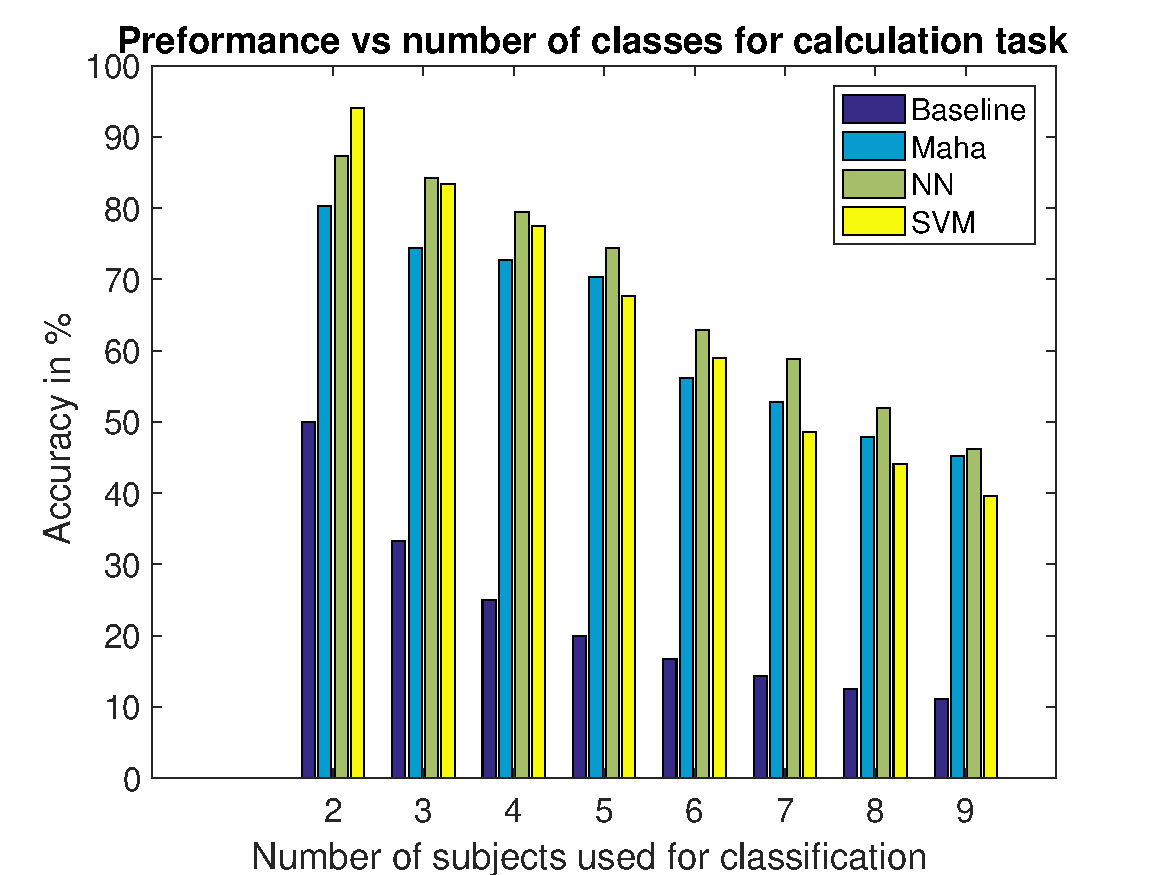
\includegraphics[width=0.9\textwidth]{Chapter-5/calc_base}
	    	\caption{Preformance vs number of classes for calculation task}
	    	\label{fig:chap5calc}
	    \end{figure}
	    
		\begin{figure}[hbtp]
	    	\centering
	    	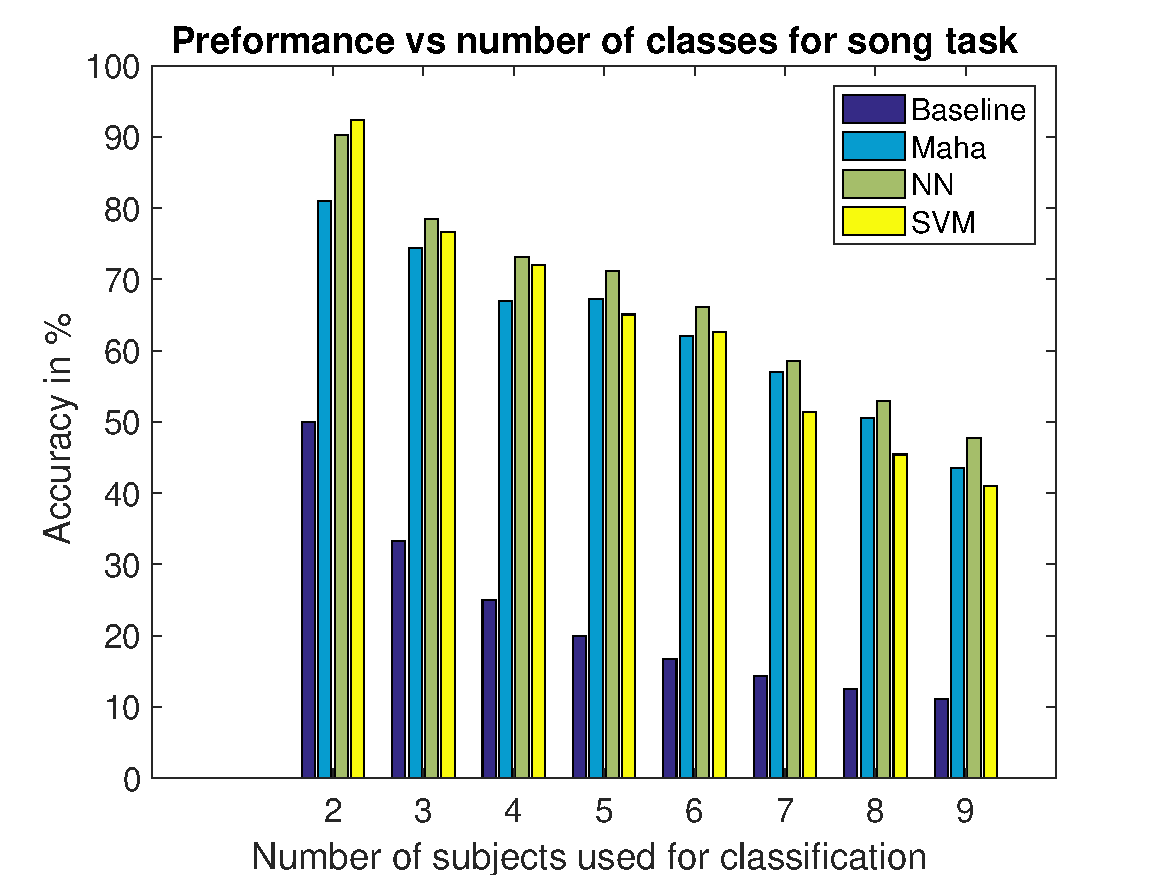
\includegraphics[width=0.9\textwidth]{Chapter-5/breath_base}
	    	\caption{Preformance vs number of classes for breathing task}
	    	\label{fig:chap5breath}
	    \end{figure}

		\begin{figure}[hbtp]
	    	\centering
	    	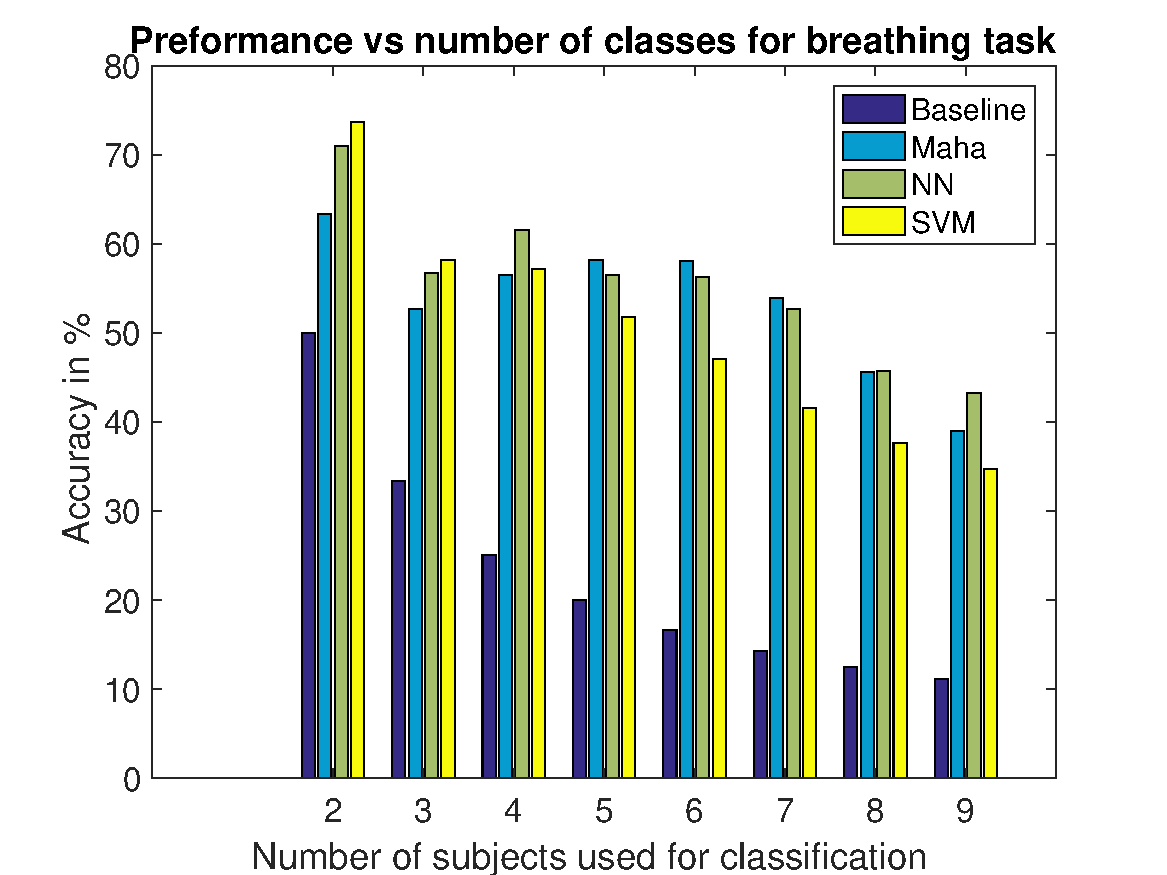
\includegraphics[width=0.9\textwidth]{Chapter-5/song_base}
	    	\caption{Preformance vs number of classes for singing task}
	    	\label{fig:chap5song}
	    \end{figure}
	    \FloatBarrier


    	

